\section[]{Subimages}
This is a fun way to look at the block action of the SVD.

%%
\begin{landscape}
\thispagestyle{empty}

\begin{table}[htdp]
\begin{center}
\begin{tabular}{ccccc}
%%
$\mat{ccc}{\A{}   & \zero & \zero \\ \zero & \A{}   & \zero \\ \zero & \zero & \A{}}  $ & = &
$\mat{ccc}{\Y{}   & \zero & \zero \\ \zero & \Y{}   & \zero \\ \zero & \zero & \Y{}}  $ & 
$\mat{ccc}{\sig{} & \zero & \zero \\ \zero & \sig{} & \zero \\ \zero & \zero & \sig{}} $ & 
$\mat{ccc}{\X{T}  & \zero & \zero \\ \zero & \X{T}  & \zero \\ \zero & \zero & \X{T}} $ \\
%%
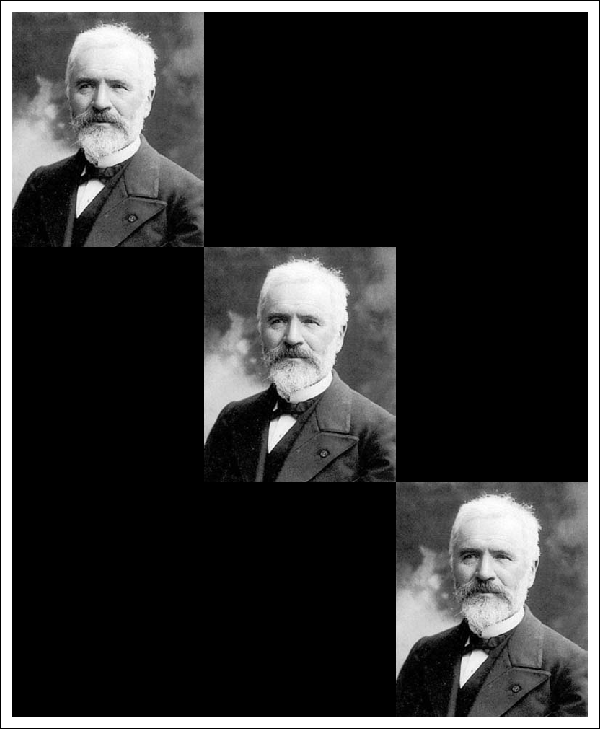
\includegraphics[ width = 1.632in ]{pdf/"ch 06"/Jordan/Jordan_subimages_diagonal} & = &
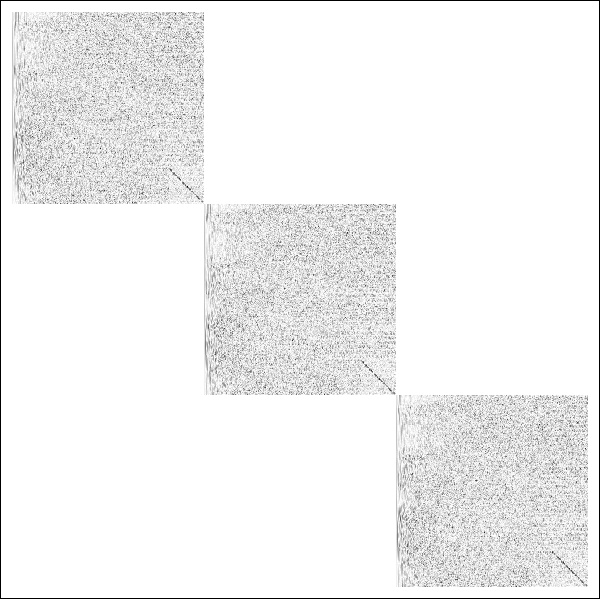
\includegraphics[ width = 2in ]    {pdf/"ch 06"/Jordan/Jordan_subimages_diagonal_Y} &

\includegraphics[ width = 1.632in ]{pdf/"ch 06"/Jordan/Jordan_subimages_diagonal_S} &
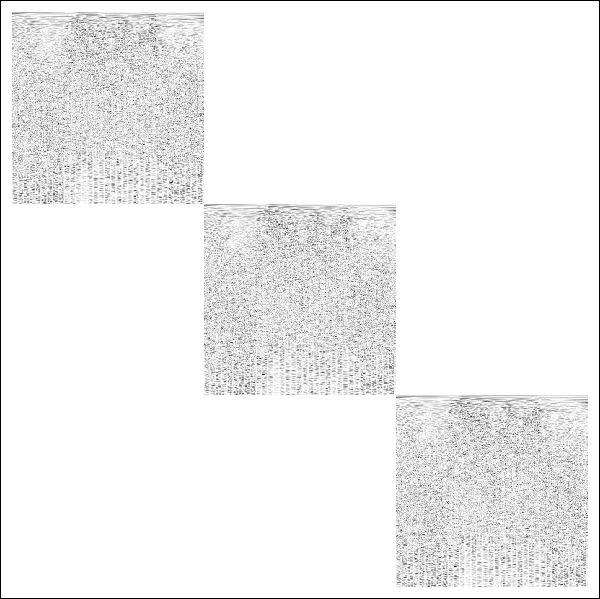
\includegraphics[ width = 1.632in ]{pdf/"ch 06"/Jordan/Jordan_subimages_diagonal_Xt}\\[20pt]
%%
$\mat{ccc}{\A{}   & \A{}  & \A{}  \\ \A{}  & \A{}  & \A{}  \\ \A{}  & \A{}  & \A{}}  $ & = &
$\mat{ccc}{\Y{}   & \zero & \zero \\ \Y{}  & \zero & \zero \\ \Y{}  & \zero & \zero} $ & 
$\mat{ccc}{\sig{} & \zero & \zero \\ \zero & \zero & \zero \\ \zero & \zero & \zero}$ & 
$\mat{ccc}{\X{T}  & \X{T} & \X{T} \\ \zero & \zero & \zero \\ \zero & \zero & \zero} $ \\
%%
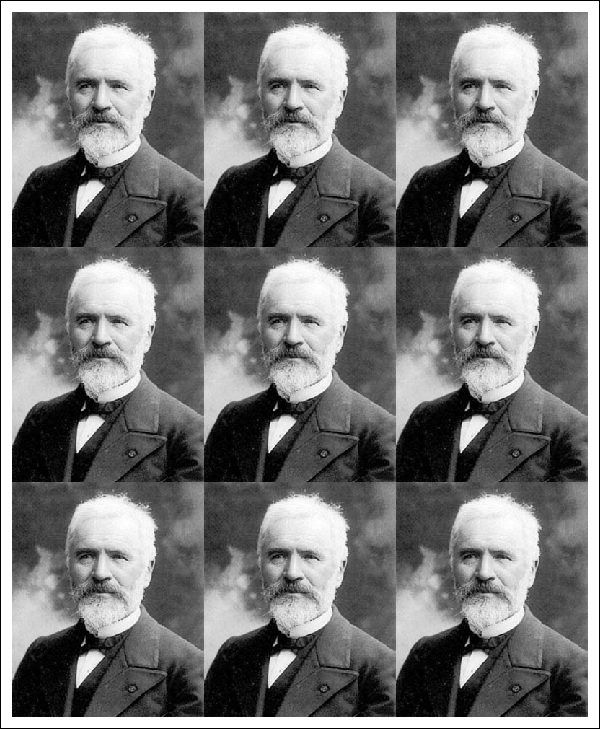
\includegraphics[ width = 1.632in ]{pdf/"ch 06"/Jordan/Jordan_subimages_9} & = &
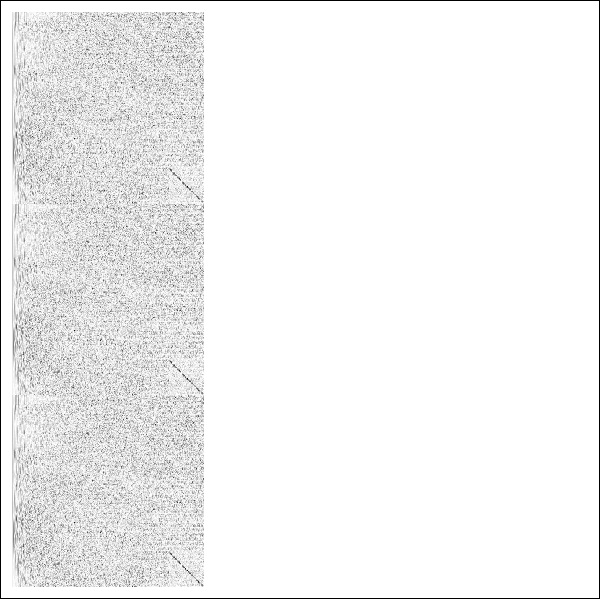
\includegraphics[ width = 2in ]    {pdf/"ch 06"/Jordan/Jordan_subimages_9_Y} &

\includegraphics[ width = 1.632in ]{pdf/"ch 06"/Jordan/Jordan_subimages_9_S} &
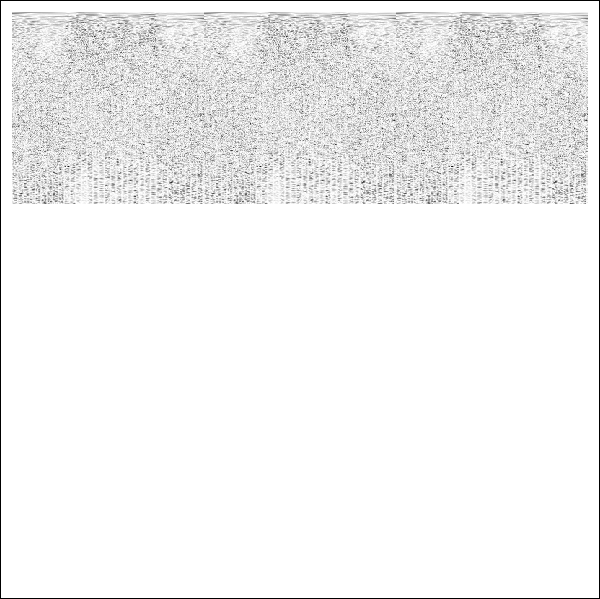
\includegraphics[ width = 1.632in ]{pdf/"ch 06"/Jordan/Jordan_subimages_9_Xt}
%%
\end{tabular}
\end{center}
\label{default}
\caption{The block block action of the SVD.}
\end{table}%

%%
\end{landscape}

\endinput